\documentclass[10pt]{article}

\usepackage[english]{babel}
\usepackage[latin1]{inputenc}
\usepackage[T1]{fontenc}
\usepackage{graphicx}
\usepackage{geometry}
\usepackage{amsmath,amssymb}
\usepackage{color}
%\usepackage{here}
\usepackage{bm}
\usepackage{epstopdf}

\begin{document}


\section{Implementation and Results}

The implementation has been done with python2.7. The svm part use the implementation of the library \textbf{scikit-learn}. We have use the implementation of TRW-S of the libraries\textbf{Opengm} and \textbf{TRW-S.1-3} you can find on the web.
\\\\
To tune the SVM parameters, we have use a per-character gridsearch over the parameter of regularisation C and the localisation of our gaussian kernel gamma. This permits us to gain a character detection gain of 10%.
\\\\
We use a simple process to test our implementation. We started with the simplest case of OCR, with a printed word on a white background, already localized. We then used harder images as our results get better.

\begin{figure}[ht!c]
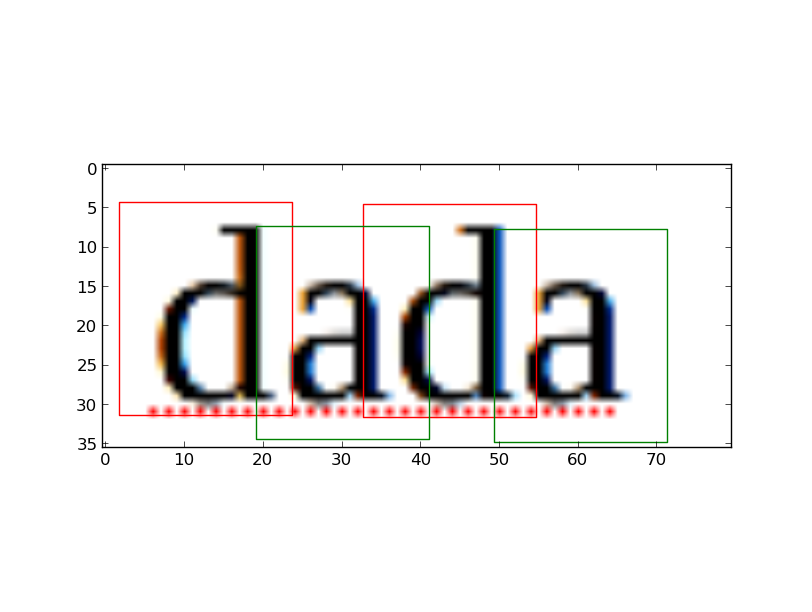
\includegraphics[width=0.3\columnwidth]{figures/dada1.png}
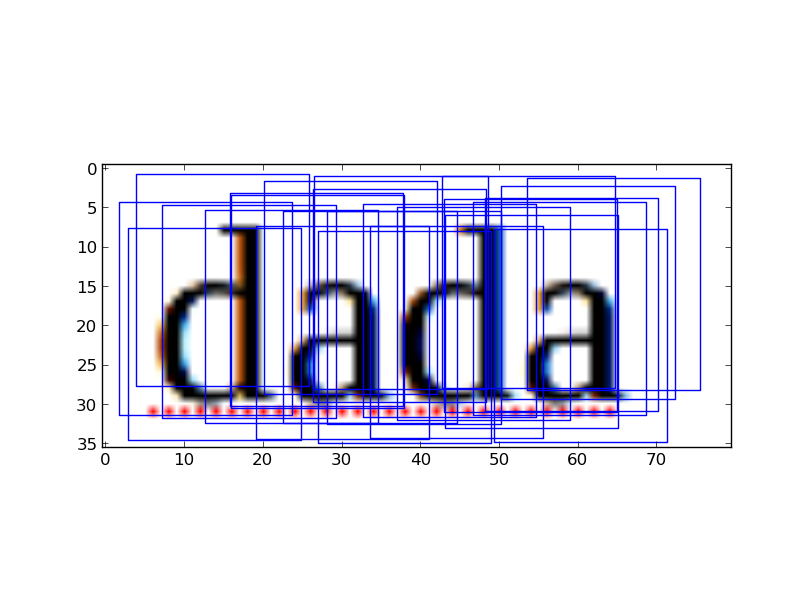
\includegraphics[width=0.3\columnwidth]{figures/dada2.png}%
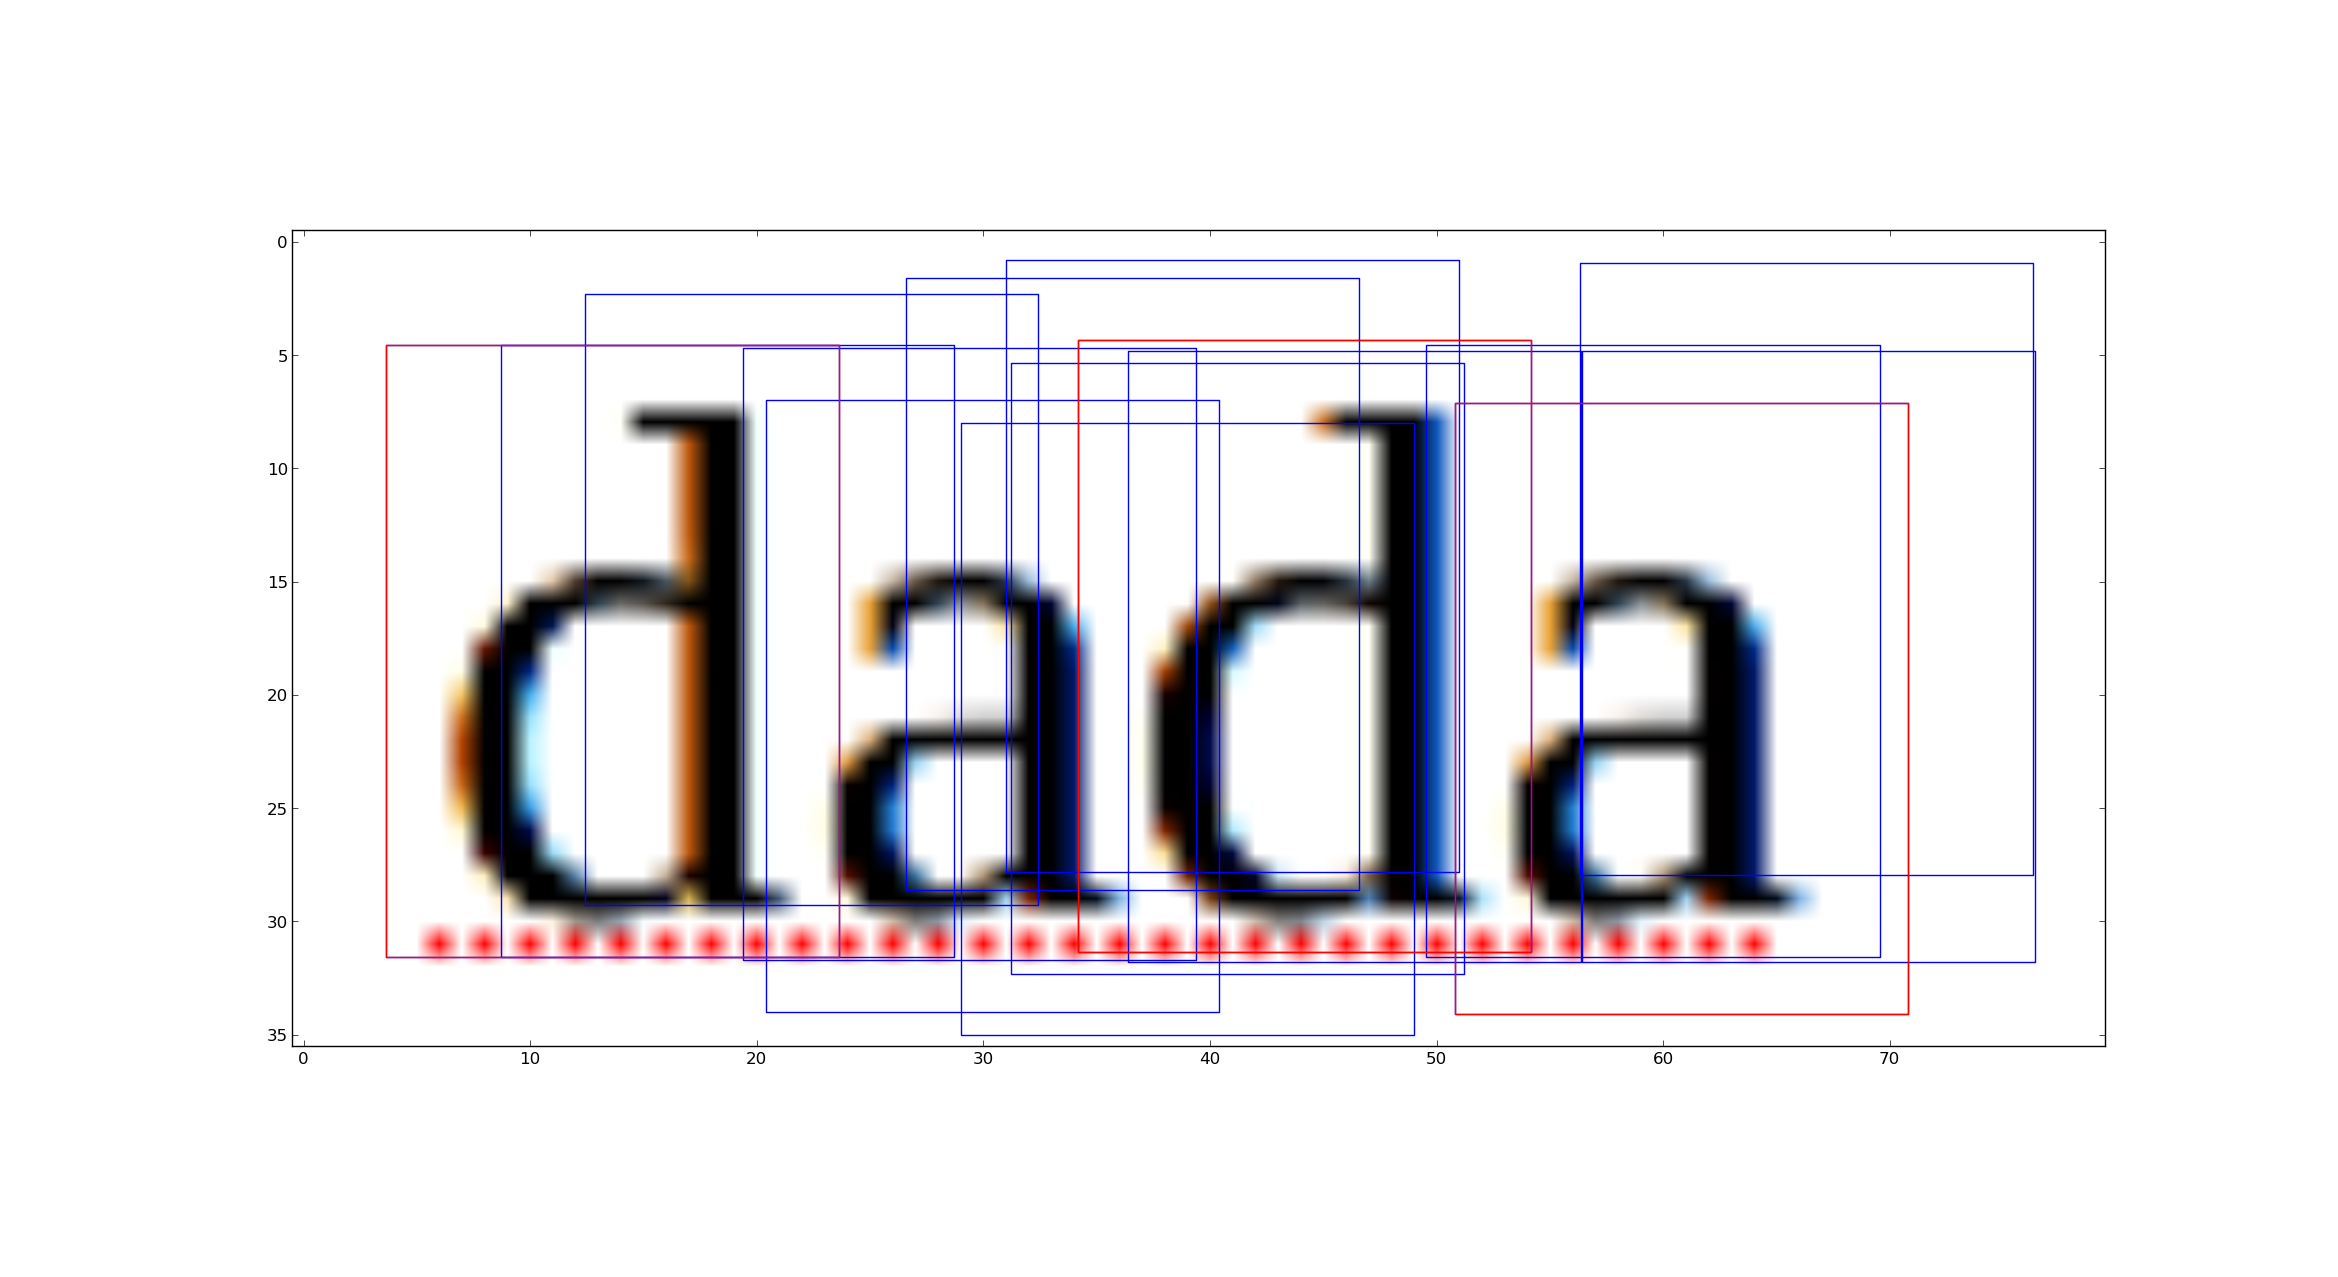
\includegraphics[width=0.3\columnwidth]{figures/dada3.png}%
\caption{Test over a artificial word 'dada'. Word retrieved: 'dda' or 'dd depending on the lexicon}
\label{dada}
\vspace{0.5cm}
\centering
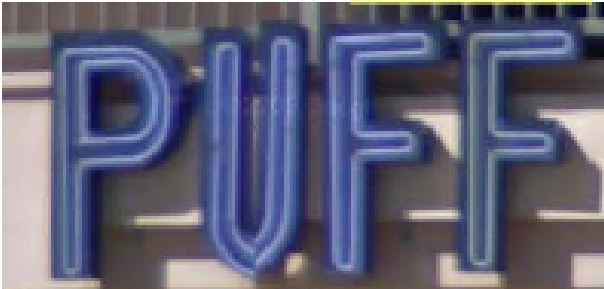
\includegraphics[width=0.4\columnwidth]{figures/puffTest.png}
\hspace{0.3cm}
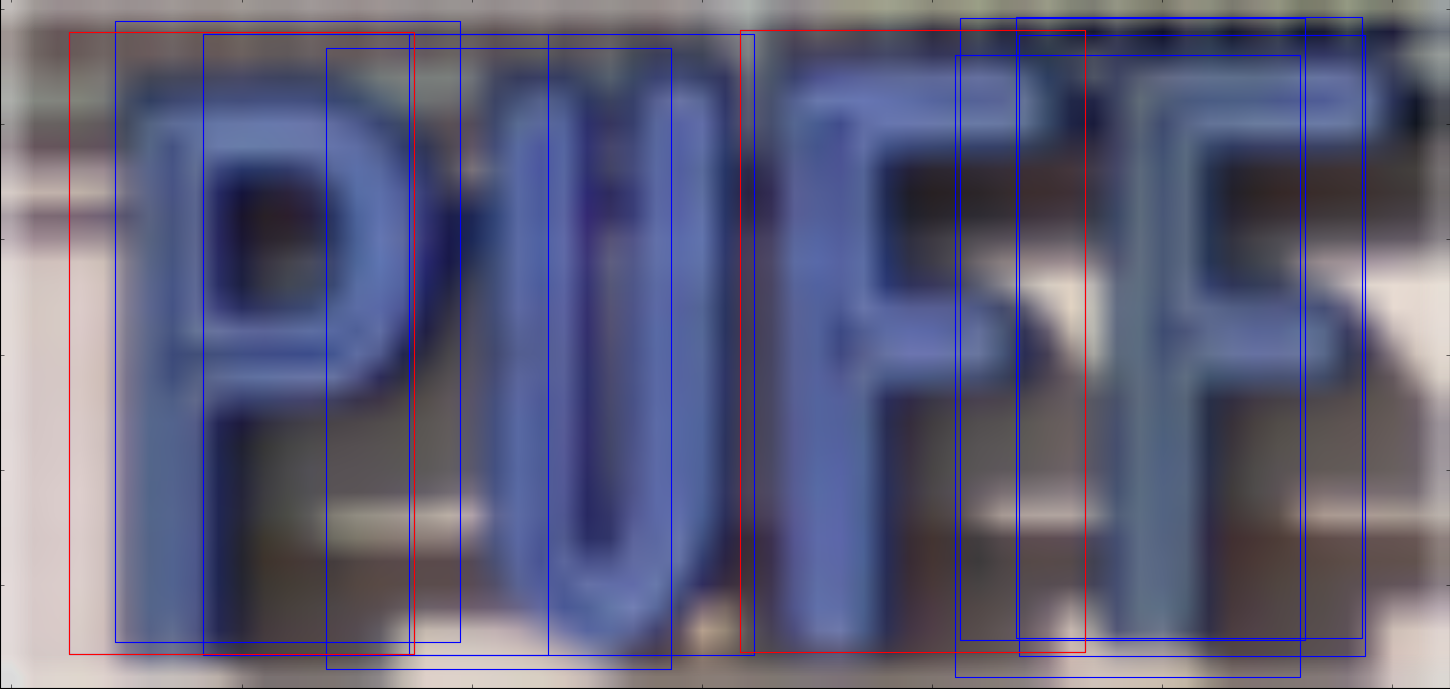
\includegraphics[width=0.4\columnwidth]{figures/puff.png}%
\caption{Natural testing word. Word retrieved: 'PE'}%
\label{Puff}
\vspace{0.5cm}
\centering
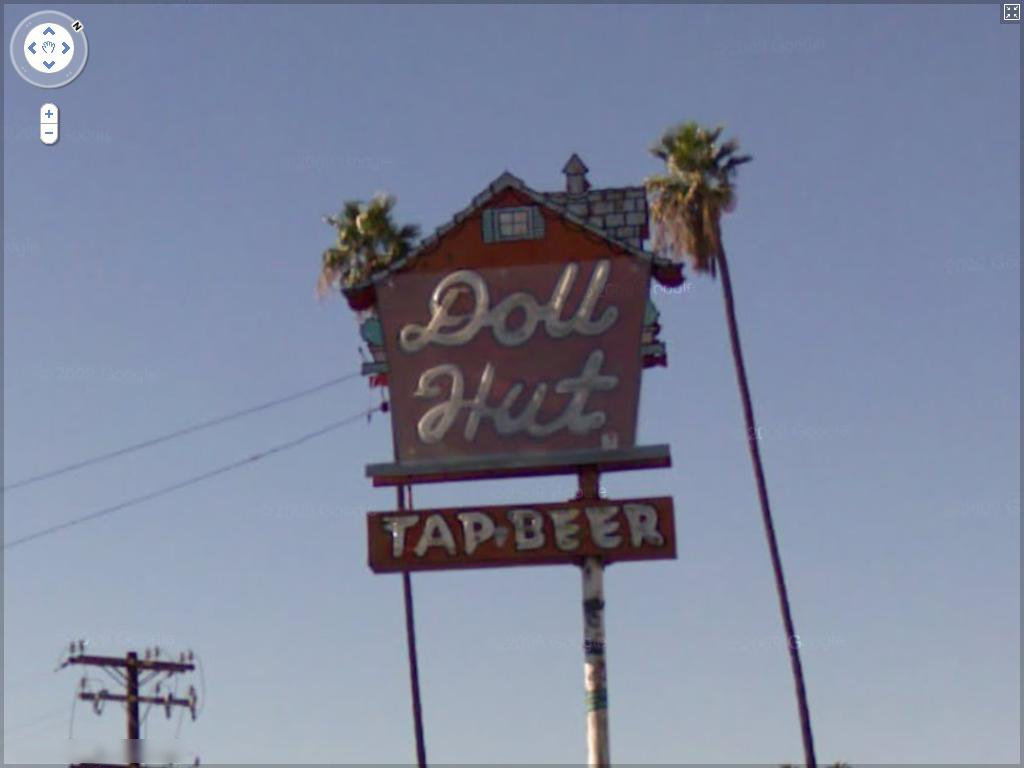
\includegraphics[width=0.4\columnwidth]{figures/00_00.jpg}
\hspace{0.3cm}
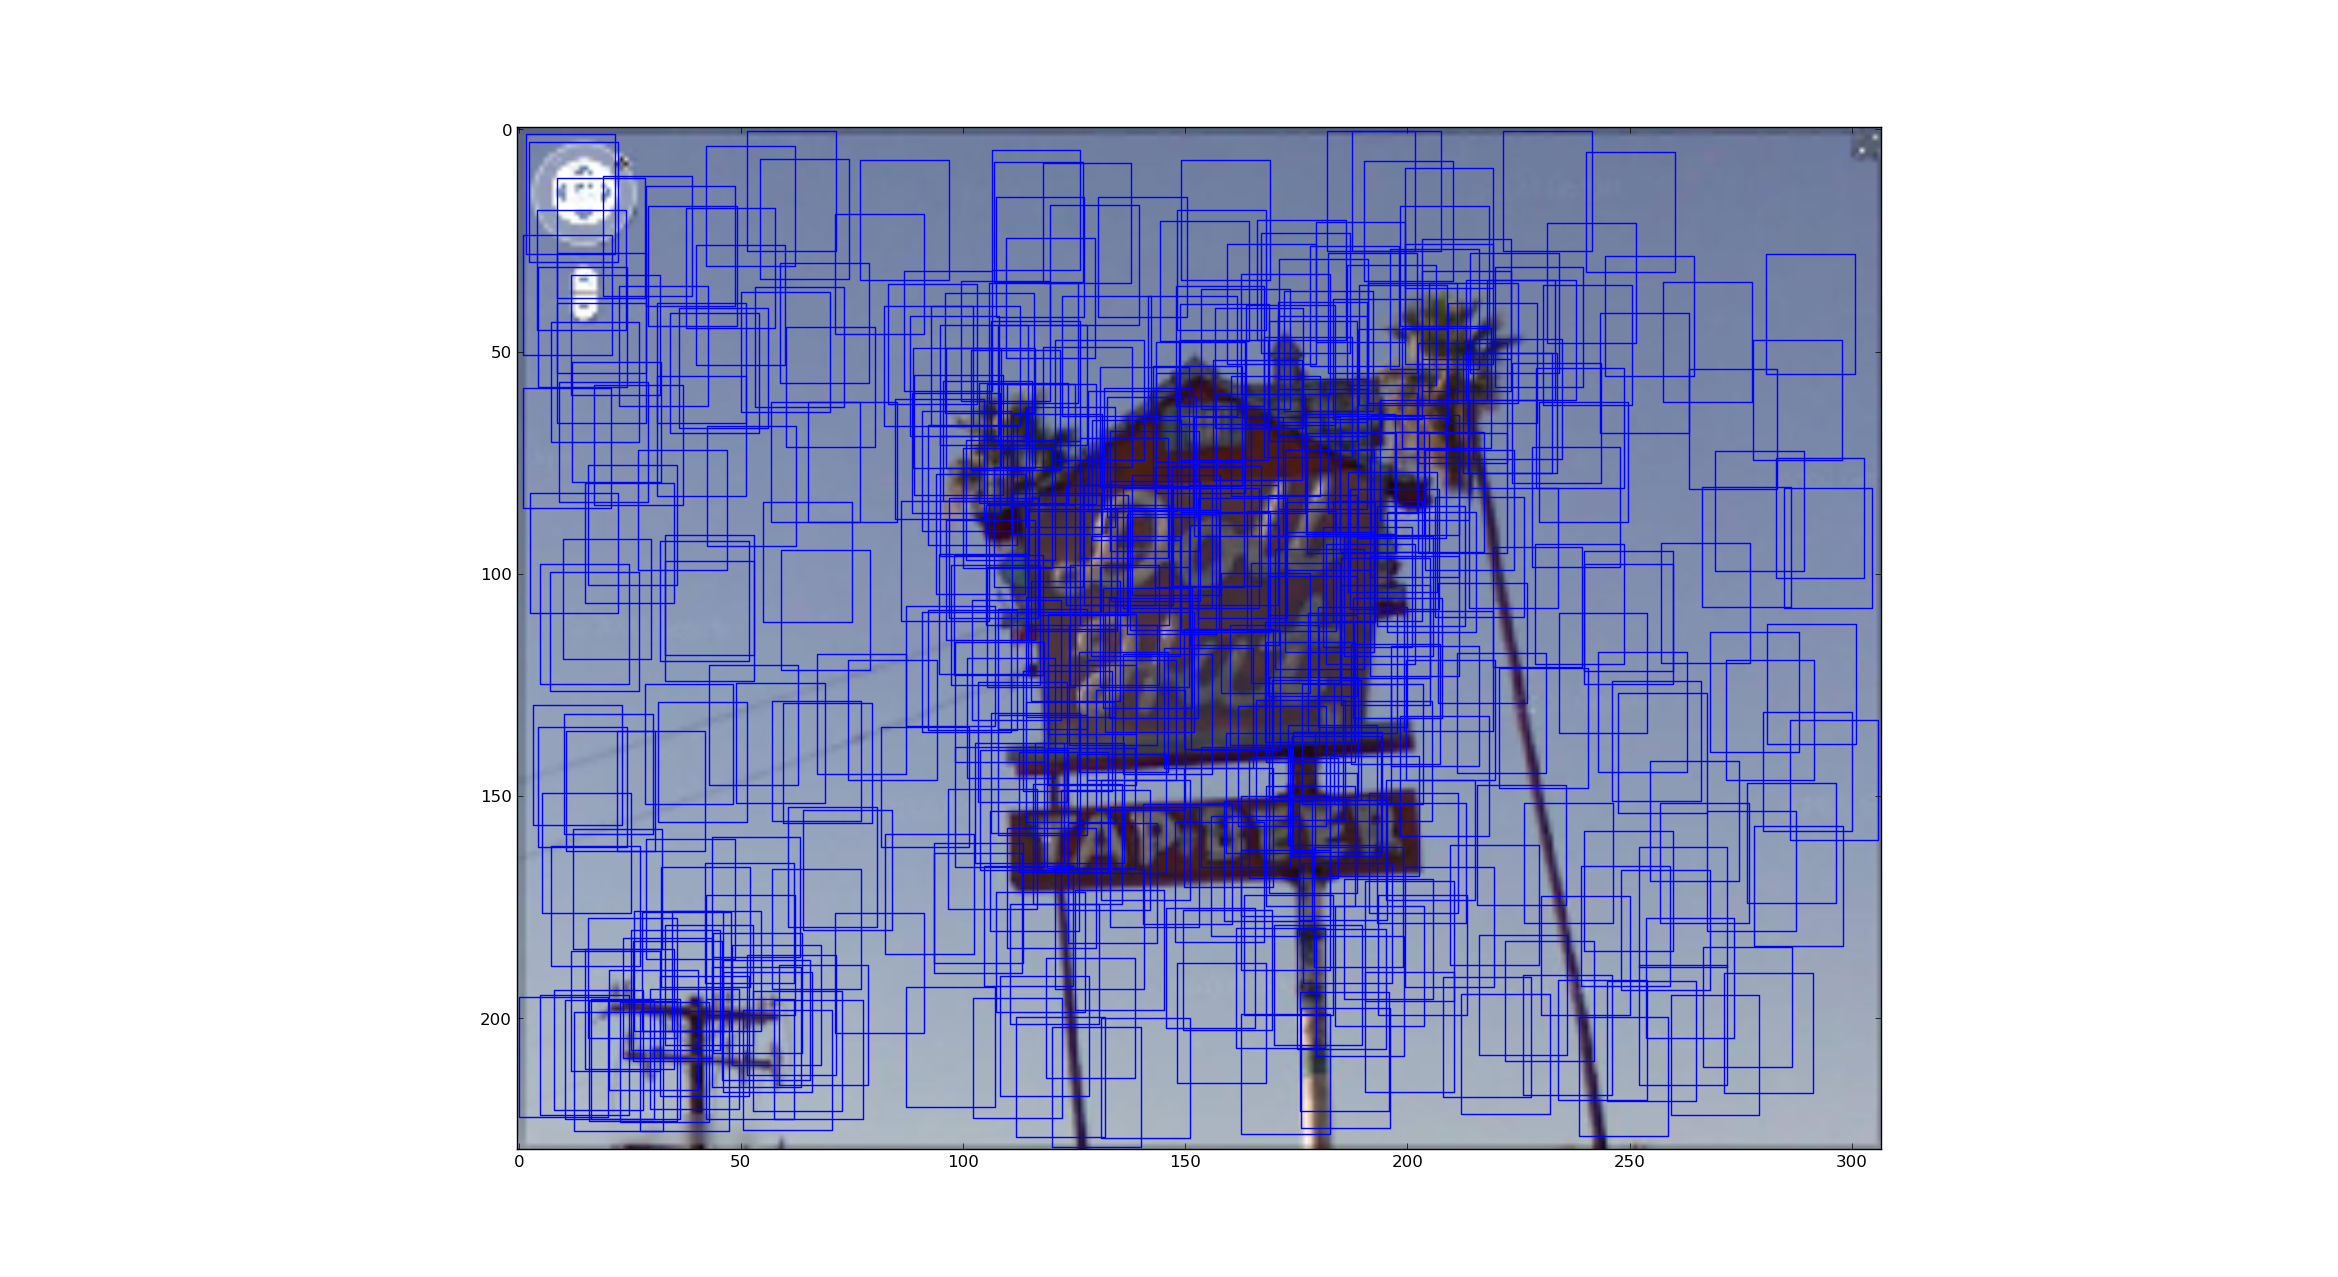
\includegraphics[width=0.4\columnwidth]{figures/beer.png}%
\caption{Natural testing image}%
\label{beer}
\end{figure}

We can see in the Fig. \ref{dada} that some there are a lot of characters are detected but we are able to select the correct ones with the graphical model. In the Fig. \ref{Puff}, we can see 2 problem. The first one is the F is detected as a E because of shade by our SVM. Then, the graphical model penalize the overlap too much and we end up with separated character instead of a word detection. The Fig. \ref{beer} show that with bigger images and multiple scale, we got a graphical model too complicated and loss the information in the noise of the observation.


\section{Improvement\\}

\begin{itemize}
\item The SVM performance is very low here even after a large cross-validation step. A first step to improve our word detection process would be to get a more robust character detection step. One idea would be to pre-select the sliding windows based on the score of a character detector model. This could still be imprecise as there is a big variability over the characters.
\\\\
\item Another observation we can make is that the model has no term in the energy that encourage the formation of words bigger than one letter in the  energy. We can often observe that the resulting word are often single separate characters whereas we are looking for a whole word.
\begin{figure}[hc!]
\centering
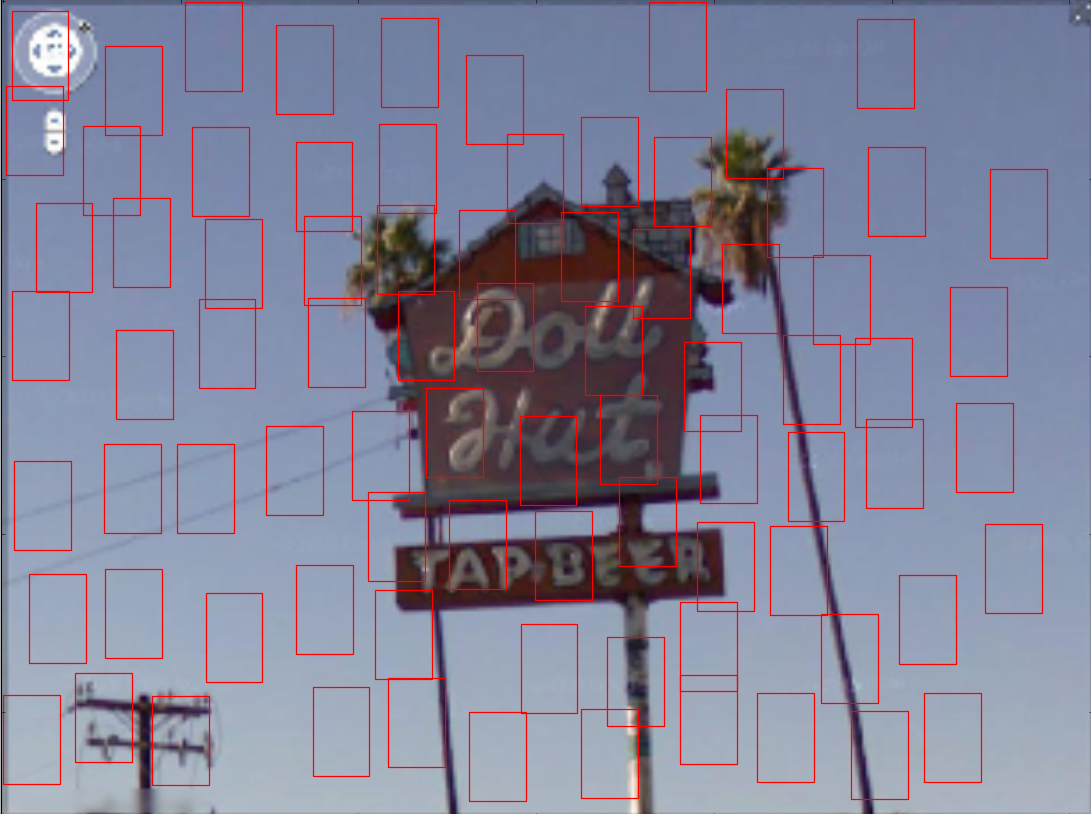
\includegraphics[width=0.3\columnwidth]{figures/beer2.png}
\caption{Spreading of the detected characters}
\end{figure}
\\\\
\item The prior we use here is a bi-gram prior. It only take into account the succession of letter. One information we are not using is the fact that a 'P' is more frequent at the begining of a word that at the end. We could thus follow the idea given in the paper \cite{Mis} to build a Node specific prior. The idea is to compute for each graphical model a prior based on the place of the node in the image and in the graphical model. But this seem to be onliy possible after a cleaning of the graphical model in the first step. We should reduce the false positive rate and then extract all the connex components of our graph to build our lexical prior in this context.
\end{itemize}




\end{document}
